% to run: lualatex ttZ_EFT.tex
\RequirePackage{luatex85}
\documentclass[tikz, border=10pt]{standalone}

\usepackage[compat=1.1.0]{tikz-feynman}

\newcommand{\Ptop}{\ensuremath{\mathrm{t}}}
\newcommand{\Pg}{\ensuremath{\mathrm{g}}}
\newcommand{\Pb}{\ensuremath{\mathrm{b}}}
\newcommand{\Pq}{\ensuremath{\mathrm{q}}}
\newcommand{\PH}{\ensuremath{\mathrm{H}}}
\newcommand{\PW}{\ensuremath{\mathrm{W}}}
\newcommand{\PZ}{\ensuremath{\mathrm{Z}}}

\makeatletter
\tikzset{
  position/.style args={#1 degrees from #2}{
    at=(#2.#1), anchor=#1+180, shift=(#1:\tikz@node@distance)
  }
}
\makeatother

\begin{document}
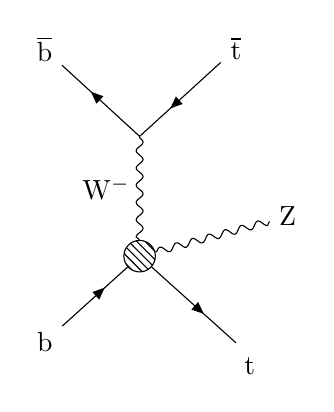
\begin{tikzpicture}
  \begin{feynman}
    \diagram [arrow size=1pt, vertical=a to b] {
      i1 [particle=\(\overline \Pb\)] -- [anti fermion] a -- [anti fermion] i2 [particle=\(\overline \Ptop\)],
      a -- [boson, edge label'=\(\PW^-\)] b [blob, minimum size=0.4cm],
      c -- [anti fermion] b -- [anti fermion] f2 [particle=\(\Pb\)],
    };

    \vertex [position=15 degrees from b] (d) {\(\PZ\)};
    \vertex [position=-45 degrees from b] (e) {\(\Ptop\)};

    \diagram* [arrow size=1pt] {
      (b) -- [boson] (d);
      % (d) -- [boson] (c) -- [fermion] (e);
    };
  \end{feynman}
\end{tikzpicture}
\end{document}
